% This is "sig-alternate.tex" V2.1 April 2013
% This file should be compiled with V2.5 of "sig-alternate.cls" May 2012
%
% This example file demonstrates the use of the 'sig-alternate.cls'
% V2.5 LaTeX2e document class file. It is for those submitting
% articles to ACM Conference Proceedings WHO DO NOT WISH TO
% STRICTLY ADHERE TO THE SIGS (PUBS-BOARD-ENDORSED) STYLE.
% The 'sig-alternate.cls' file will produce a similar-looking,
% albeit, 'tighter' paper resulting in, invariably, fewer pages.
%
% ----------------------------------------------------------------------------------------------------------------
% This .tex file (and associated .cls V2.5) produces:
%       1) The Permission Statement
%       2) The Conference (location) Info information
%       3) The Copyright Line with ACM data
%       4) NO page numbers
%
% as against the acm_proc_article-sp.cls file which
% DOES NOT produce 1) thru' 3) above.
%
% Using 'sig-alternate.cls' you have control, however, from within
% the source .tex file, over both the CopyrightYear
% (defaulted to 200X) and the ACM Copyright Data
% (defaulted to X-XXXXX-XX-X/XX/XX).
% e.g.
% \CopyrightYear{2007} will cause 2007 to appear in the copyright line.
% \crdata{0-12345-67-8/90/12} will cause 0-12345-67-8/90/12 to appear in the copyright line.
%
% ---------------------------------------------------------------------------------------------------------------
% This .tex source is an example which *does* use
% the .bib file (from which the .bbl file % is produced).
% REMEMBER HOWEVER: After having produced the .bbl file,
% and prior to final submission, you *NEED* to 'insert'
% your .bbl file into your source .tex file so as to provide
% ONE 'self-contained' source file.
%
% ================= IF YOU HAVE QUESTIONS =======================
% Questions regarding the SIGS styles, SIGS policies and
% procedures, Conferences etc. should be sent to
% Adrienne Griscti (griscti@acm.org)
%
% Technical questions _only_ to
% Gerald Murray (murray@hq.acm.org)
% ===============================================================
%
% For tracking purposes - this is V2.0 - May 2012

\documentclass[conference]{IEEEtran}

\usepackage[
    colorlinks=true,
    linkcolor=black,
    citecolor=black,
    filecolor=black,
    urlcolor=black,
    bookmarks=true,
    bookmarksopen=true,
    bookmarksopenlevel=3,
    plainpages=false,
    pdfpagelabels=true,
    hypertexnames=false
]{hyperref}
\usepackage{cite}
\usepackage{amsmath}
\usepackage{listings}
\usepackage{scalefnt}
\usepackage{color}
\usepackage{tikz}
\usepackage{ifthen}
\usepackage{pgfplots}
\usepackage{eqparbox}

\usetikzlibrary{automata}
\usetikzlibrary{calc}
\usetikzlibrary{shapes,backgrounds}
\usetikzlibrary{shapes.geometric}
\usetikzlibrary{positioning}
\usetikzlibrary{arrows}



\renewcommand{\topfraction}{0.95}
\renewcommand{\bottomfraction}{0.95}
\renewcommand{\textfraction}{0.1}
%\renewcommand{\textfraction}{0.0}
\renewcommand{\floatpagefraction}{0.75}
%\renewcommand{\floatpagefraction}{1.0}

%%%%%%%%%%%%%%%%%%%%%%%%%%%%%%%%%%%%%%%%%%%%%%%%%%%%%%%%%%%%%%%%%%%%%%%%%%%%%%
% Avoid Hurenkinder und Schusterjungen
%%%%%%%%%%%%%%%%%%%%%%%%%%%%%%%%%%%%%%%%%%%%%%%%%%%%%%%%%%%%%%%%%%%%%%%%%%%%%%
\clubpenalty = 10000
\widowpenalty = 10000 \displaywidowpenalty = 10000
\interdisplaylinepenalty=2500

% X10 language definition
\lstdefinelanguage{x10}{
    morekeywords = {
        abstract, as, assert, async, at,
        atomic, break, case,
        catch, class, clocked, continue, def,
        default, do, else, extends, false,
        final, finally, finish, for, goto,
        haszero, here, if, implements, import,
        in, instanceof, interface, native, new,
        null, offer, offers, operator, package,
        private, property, protected, public, return,
        self, static, struct, super, switch,
        this, throw, transient, true, try,
  basicstyle=
  numberstyle=
        type, val, var, void, when,
        while
    },
    morecomment = [l]{//},
    morecomment = [s]{/*}{*/},
    morestring = [b]",
}

\definecolor{keywordcolor}{RGB}{0,0,127}
\definecolor{commentcolor}{RGB}{0,127,0}
\definecolor{stringcolor}{RGB}{127,0,0}
\definecolor{whitesmoke}{RGB}{246,246,246}

% global listings style
\lstset{
    % language
    language=x10,
    % code style
    basicstyle=\ttfamily \scalefont{.8},%\scriptsize\sffamily,
    keywordstyle=\color{keywordcolor}\bfseries,
    commentstyle=\color{commentcolor}\itshape,
    stringstyle=\color{stringcolor},
    breaklines=true,
%    tabsize=2,
    % number style
    numbers=left,
    numberstyle=\ttfamily\scalefont{.8},%\scriptsize\sffamily,
    numbersep=2pt,
    lineskip=-1pt,
    xleftmargin=9pt,
%    framexleftmargin=10pt,
    % box style
    %backgroundcolor=\color{whitesmoke},
    captionpos=b
}

\newcommand{\todo}[1]{{\color{red}\ttfamily #1}}


\begin{document}

\IEEEoverridecommandlockouts
\title{SWE-X10: Simulating shallow water waves with lazy activation of patches using ActorX10}


\author{
    \IEEEauthorblockN{Alexander P{\"o}ppl and Michael Bader}
    \IEEEauthorblockA{
        Technical University of Munich\\
        Boltzmannstra{\ss}e 3, 85748 Garching bei M{\"u}nchen, Germany\\
        Email: \{poeppl, bader\}@in.tum.de
    }
    \and
    \IEEEauthorblockN{Tobias Schwarzer and Michael Gla{\ss}}
    \IEEEauthorblockA{
        Friedrich-Alexander-Universit\"at Erlangen-N\"urnberg (FAU)\\ 
        Cauerstra{\ss}e 11, 91058 Erlangen, Germany\\
        Email: \{tobias.schwarzer, michael.glass\}@fau.de
    }
%    \IEEEauthorblockN{Michael Gla{\ss}}
%    \IEEEauthorblockA{
%    
%    }

}
%\numberofauthors{2} 
%
%\author{
% 1st. author
%    \alignauthor
%    Alexander P\"oppl, Michael Bader\\
%    \affaddr{Technical University of Munich}\\
%    \affaddr{Boltzmannstra{\ss}e 3}\\
%    \affaddr{85748 Garching bei M\"unchen, Germany}\\
%    \email{\{poeppl,bader\}@in.tum.de}
% 2nd. author
%    \alignauthor
%    Tobias Schwarzer, Michael Gla\ss\\
%    \affaddr{Friedrich-Alexander-Universit\"at Erlangen-N\"urnberg (FAU)}\\
%    \affaddr{Cauerstra{\ss}e 11, 91058 Erlangen, Germany}\\
%    \email{\{tobias.schwarzer,michael.glass\}@fau.de}
%}
\maketitle
\begin{abstract}
We present an efficient Finite Volume solver for the shallow water equations using an actor extension of the 
X10 programming language, ActorX10, as programming model. Each actor is assigned to a 
Cartesian patch of the computational grid.  
Using the actor's finite state machine to control patch updates, we realize \emph{lazy activation} 
of patches, only when a propagating wave enters the respective patch. 
Overlapping of communication and computation in the fully non-central actor-based control, 
as well as careful optimization (esp.\ vectorization) of kernels leads to high performance 
and parallel efficiency in shared and distributed memory. 
Benefits of lazy activation are demonstrated via reduced CPU hours for a benchmark scenario.
\end{abstract}

\begin{IEEEkeywords}
High performance computing, parallel programming, performance analysis, computer languages

\end{IEEEkeywords}

\IEEEpubid{
    ESPM2 2016; Salt Lake City, Utah, USA; November 2016
    978-1-5090-3858-9/16/\$31.00 \copyright 2016 IEEE
}

% The code below should be generated by the tool at
% http://dl.acm.org/ccs.cfm
% Please copy and paste the code instead of the example below. 
%
 %\begin{CCSXML}
%<ccs2012>
%<concept>
%<concept_id>10002950.10003705.10011686</concept_id>
%<concept_desc>Mathematics of computing~Mathematical software performance</concept_desc>
%<concept_significance>500</concept_significance>
%</concept>
%<concept>
%<concept_id>10010147.10010169.10010170</concept_id>
%<concept_desc>Computing methodologies~Parallel algorithms</concept_desc>
%<concept_significance>500</concept_significance>
%</concept>
%<concept>
%<concept_id>10010147.10010169.10010175</concept_id>
%<concept_desc>Computing methodologies~Parallel programming languages</concept_desc>
%<concept_significance>500</concept_significance>
%</concept>
%</ccs2012>
%\end{CCSXML}

%\ccsdesc[500]{Mathematics of computing~Mathematical software performance}
%\ccsdesc[500]{Computing methodologies~Parallel algorithms}
%\ccsdesc[500]{Computing methodologies~Parallel programming languages}


%
% End generated code
%

%
%  Use this command to print the description
%
%\printccsdesc

%\keywords{PGAS languages; X10; hyperbolic partial differential equations; shallow water equations; actor-based programming model}

%%%%%%%%%%%%%%%%%%%%%%%%%%%%%%%%%%%%%%%%%%%%%%%%%%%%%%%%%%%%%%%%%%%%%%%%%%%%%%%%%%%%%%%%%%%%
%%%%%%%%%%%%%%%%%%%%%%%%%%%%%%%%%%%%%%%%%%%%%%%%%%%%%%%%%%%%%%%%%%%%%%%%%%%%%%%%%%%%%%%%%%%%
%% BEGIN MAIN MATTER
%%%%%%%%%%%%%%%%%%%%%%%%%%%%%%%%%%%%%%%%%%%%%%%%%%%%%%%%%%%%%%%%%%%%%%%%%%%%%%%%%%%%%%%%%%%%
%%%%%%%%%%%%%%%%%%%%%%%%%%%%%%%%%%%%%%%%%%%%%%%%%%%%%%%%%%%%%%%%%%%%%%%%%%%%%%%%%%%%%%%%%%%%

\section{Introduction}

\IEEEpubidadjcol
\IEEEPARstart{A}{ssigning} dynamic work load to heterogeneous and dynamically changing hardware is likely to evolve into a key challenge in scientific computing. 
Modern architectures evolve towards many-core designs, where accelerator techniques (consider GPGPUs or Xeon Phi co-processors), dynamic frequency scaling and temporary selective use (or shut-down) of parts of the CPU (``dark silicon'') characterize dynamic availability of resources. 
Similar, large-scale applications need to dynamically invest degrees of freedom where they lead to the largest gain in accuracy, leading to dynamic requirements of resources on the application side. 
Nevertheless, the predominant programming models in scientific computing primarily target a fixed set of resources -- typically a given number of compute nodes -- which is to be used as efficiently as possible.  

In this paper, we present the proxy application SWE-X10 (earlier version shown in the extended abstract \cite{poeppl2016swex10}), which follows an \emph{actor approach} towards more dynamic use of resources. 
We show how finite state machines, as part of an actor-oriented parallel programming model, can be used to identify parts of the computational domain that are not updated: 
following a ``lazy activation'' paradigm, respective compute resources could remain idle until needed. 
In addition, the actor approach allows Cartesian grid patches to propagate in time without global control.  
The implementation is based on the APGAS language X10 and uses the actor extension ActorX10~\cite{roloff2016actorx10}. 
We demonstrate the general feasibility of ``lazy activation'' and evaluate the parallel efficiency of the X10 implementation.

While the implementation is currently limited to uniform Cartesian grids, we envisage a block-adaptive version as the next step, where multilevel grids with different resolutions are used. 
Lazy activation would then be used for fine-grid levels. 
The actor approach also enables the use of automatic methods for design-time characterization, as known from embedded computing:
Using fast analysis techniques or short sample simulations, such approaches not only allow for parameter optimization wrt.\ various parameters such as patch sizes, distributions, or load balancing, but also explore the different trade-offs between performance, the number of used components, energy consumption etc.

In the following, we first introduce the shallow water proxy application SWE-X10 (\autoref{sec:math}) 
and provide details on the actor model implemented in ActorX10 (\autoref{sec:actor}).
In \autoref{sec:impl}, we discuss the actor implementation and performance issues of SWE-X10. 
Section~\ref{sec:results} evaluates parallel performance and potential gains from lazy activation. 
 
%%%%%%%%%%%%%%%%%%%%%%%%%%%%%%%%%%%%%%%%%%%%%%%%%%%%%%%%%%%%%%%%%%%%%%%%%%%%%%%%%%%%%%%%%%%%

\section{Mathematical Background}
\label{sec:math}
%\begin{itemize}
%    \item Based on SWE, solver for Shallow Water Equations
%    \item Hyperbolic PDE, changes propagate outwards from initial disturbance of steady state.
%    \item Discretization using explicit a Finite Volume scheme with explicit Euler time stepping.
%    \item Piecewise constant regular grid cells.
%\end{itemize}

In this work, we focus on modeling based on hyperbolic partial differential equations (PDEs), which are characterized by their ``wave-type'' solutions that propagate signals at finite propagation speed.
Initial disturbances in parts of the domain will not effect the rest of the domain (beyond an ``event horizon'') immediately -- an effect we will utilize later to avoid the computation of zero-updates. 
As an example for a particular hyperbolic PDE system, we focus on the shallow water equations.
\IEEEpubidadjcol
%\newpage
\subsection{The Shallow Water Equations}
\label{sec:sweq}

The shallow water equations are a nonlinear system of conservation laws for depth and momentum that is commonly used to simulate, for example, the propagation of tsunamis, as well as, with additional source terms, the inundation of coastal regions~\cite{leveque2011tsunami}.
They can be derived from the three-dimensional Navier-Stokes equations by averaging over the depth dimension.
In its two-dimensional form,
\begin{align}
    \label{eq:numeric:shallow}
    \begin{bmatrix}
        h\\hu\\hv
    \end{bmatrix}_t + 
    \begin{bmatrix}
        hu\\hu^2+\frac{1}{2}gh^2\\huv
    \end{bmatrix}_x +
    \begin{bmatrix}
        hv\\huv\\hv^2+\frac{1}{2}gh^2
    \end{bmatrix}_y =
    \begin{bmatrix}
        0\\
        -ghB_x\\
        -ghB_y
    \end{bmatrix},
\end{align}
%
$h(x,y,t)$ is the height of the water column at position $(x,y)$ and time $t$;
the velocities in the two spacial dimensions are described by $u(x,y,t)$ and $v(x,y,t)$, and $g$ is the gravitational constant.
Source terms on the right-hand side model additional effects, such as the influence of terrain above (during inundation) and below sea level.
The latter, i.e., the elevation of the ocean floor, is often referred to as \emph{bathymetry} data, here denoted as $B(x,y)$. \\

\subsection{The Finite Volume Model}
\label{sec:numerics}
The numerical model used for SWE-X10 is based on the SWE package, a hybrid OpenMP/MPI proxy application written in C++~\cite{breuer2012teaching}. 
Both packages follow a classical Finite Volume approach, as suggested by LeVeque et al.~\cite{leveque2011tsunami}. 
The simulation domain is discretized on an equidistant Cartesian grid. 
Each cell $i,j$ stores a vector of  cell-averaged quantities, 
$Q^{(n)}_{i,j} = [h^{(n)}_{i,j},(hu)^{(n)}_{i,j}, (hv)^{(n)}_{i,j}, b^{(n)}_{i,j}]$, 
at time step $t_n$.
Starting at initial time $t_0$, the unknowns are successively updated according to the following update scheme:
%
\begin{align}
    \label{eq:update_scheme}
    Q^{(\text{n}+1)}_{i,j} = Q^{\text{(n)}}_{i,j} &- \frac{\Delta t}{\Delta x}\left(\mathcal{A}^+\Delta Q^{(\text{n})}_{i-\frac{1}{2}, j} + \mathcal{A}^-\Delta Q^{(\text{n})}_{i+\frac{1}{2}, j} \right) \\
    &-\frac{\Delta t}{\Delta y}\left(\mathcal{B}^+\Delta Q^{(\text{n})}_{i, j-\frac{1}{2}}+\mathcal{B}^-\Delta Q^{(\text{n})}_{i, j+\frac{1}{2}} \right),\notag
\end{align}
%
where $\Delta t$ is the time step size, and $\Delta x$ and $\Delta y$ denote the cell size in $x$ and $y$ direction.

$\mathcal{A}^\pm\Delta Q^{(\text{n})}_{i\pm\frac{1}{2}, j}$ and 
$\mathcal{B}^\pm\Delta Q^{(\text{n})}_{i, j\pm\frac{1}{2}}$ 
are so-called \emph{net updates} computed for the horizontal and vertical cell edges, respectively.
They are obtained from the approximate solution of respective Riemann problems at the edges, and reflect the transport of mass and momentum between adjacent cells during a single time step. 
%% -> MB: omitted details on Riemann solvers; not necessary
%The solution to these is usually not computed analytically.
%While it is possible to do so, it is expensive to compute in the non-linear case.
%Moreover, the positive effect of using precise solver is negated by the Finite volume discretization, which introduces errors compared to a continuous solution in each time step. 
%Instead, approximate solvers are used.
SWE-X10 supports two different approximate solvers: the f-Wave~\cite{bale2003wavePropagation} solver is a relatively simple solver that produces good results for wave propagation across the open ocean. 
It is not, however, able to model inundation, and thus treats coast lines as a wall boundary.
The HLLE solver~\cite{einfeldt1988godunov,Harten1997} handles inundation at the cost of a moderate increase in computational complexity. 
Both implementations have been tailored to allow auto-vectorization by the compiler. 
%There exist other solvers~\cite{bader2014vectorization} that are able to model observed behavior even more precisely, but we found the HLLE solver to be a good trade-off between precision of the solutions provided and its computational complexity.

The finite propagation speed of an initial perturbance is reflected in the update scheme (\autoref{eq:update_scheme}), as it only considers the four direct neighbors of a cell. 
Propagation is therefore limited to one cell size per time step, which poses a restriction to the time step size $\Delta t$ (the well-known CFL condition). 
In typical implementations, cells are updated regardless of a perturbation in their neighboring cells, 
which leads to a large number of ``trivial'' zero-updates that use computing resources unnecessarily.

%%%%%%%%%%%%%%%%%%%%%%%%%%%%%%%%%%%%%%%%%%%%%%%%%%%%%%%%%%%%%%%%%%%%%%%%%%%%%%%%%%%%%%%%%%%%

\section{Actor Model}
\label{sec:actor}

The actor model is a computational model first described by Hewitt~\cite{hewitt1973actor} (in the context of artificial intelligence) and later formalized by Agha~\cite{agha1985actors}.
Essentially, an actor may be described as a thread of execution with a state attached to it. 
Actors execute their code independently and without explicit synchronization.
Collaboration between actors may be attained by explicit messages through statically defined communication channels, or at the start of the program execution.
This structure allows for a very low amount of coupling. As communication is handled by the actor framework, actors only need to specify their communication interfaces, and how to react to data being available to them.
The concrete implementation of the actors is encapsulated from the other actors in the actor graph.

SWE-X10 uses the actor model where control is realized by means of Finite State Machines (FSMs) -- resembling the FunState~\cite{STGZET:2001} Model-of-Computation -- to implement a distributed and locally coordinated time stepping scheme.
In the following section we will give a quick introduction of the actor model as implemented in the ActorX10 actor library~\cite{roloff2016actorx10}, which was used to implement SWE-X10.

\subsection{Components}
\label{sec:actor:components}
The basic building blocks of the actor-based computational model are \emph{channels}, \emph{ports}, and \emph{actors}.
These components are arranged in the \emph{actor graph}.
In the following, we give a short definition and outline of each of these components' functionalities.

Actors may be described abstractly by the tuple $a=(I, O, F, R)$ containing the set of incoming ports $I$ for receiving data, the set of outgoing ports $O$ for sending data, and the set of functions $F$ callable in the course of the firing of the actor's finite state machine $R$. 
The state machine $R = (Q, q_0, T)$ consists of a finite set of states $Q$, an initial state $q_0\in Q$ and a set of transitions $T$ between these states.
It is called whenever there is a change in one of the actor's ports, which effectively leads to an inversion of control.
The application developer only specifies how to react to the changes, but has no control over their timing or their sequence of their arrival.
The order in which events are handled may be manipulated using states in the state machine.
Each transition also defines guard functions that determine whether a transition is triggered, and the functions that will be executed when the transition is triggered.
Finally, the number of data elements required to perform the transition and the necessary space needed to store the resulting output in the corresponding outgoing ports is specified.

Ports are the typed facades the actors utilize for their communications.
Each port has a type describing the kind of data that may be sent or received through it, an actor it belongs to and a channel to which it is assigned dynamically at application run time. 
Incoming ports offer facilities to query for the availability of data or to read one or more elements from it.
Outgoing ports offer to query the channel's remaining capacity and functionality to write data to it.
Channels are unidirectional connections between exactly one outgoing (writing) and one incoming (reading) port. 
They are implemented using FIFO semantics in order to preserve the sequence in which the messages have been sent.

\subsection{Using the ActorX10 library}
\label{sec:actor:example}
The ActorX10 library is organized as a white-box framework.
To use the actor functionality, application developers have to subclass the \texttt{Actor} class and override the \texttt{act()} method, which will be called whenever there is a change at any of the registered ports.
To register a port, one calls the generic \texttt{newInPort[T](String)} method for \texttt{InPort}s and the \texttt{newOutPort[T](String)} method for \texttt{OutPort}s.

In \autoref{sec:actor:components}, we stated that transitions of the actor FSM may be protected by guards, i.e.\ Boolean functions that depend on the values of the inputs available in the ports. 
Therefore, the \texttt{InPort}s provide facilities to query the amount of available data items -- using the overloaded \texttt{operator()} -- as well as to perform destructive as well as non-destructive reads from the channel using the \texttt{read():T} and \texttt{peek():T} methods.

\begin{figure}
    \centering
    \begin{lstlisting}
public class SimulationActor extends Actor {
  public val leftIn = newInPort[Data]("left");
  public val rightIn = newInPort[Data]("right");
  public val leftOut = newOutPort[Data]("left");
  public val rightOut = newOutPort[Data]("right");

  public def this(name:String) {
    super(name);
  }
  
  public def act() {
    if (leftIn() && rightIn() 
          && leftOut() && rightOut()) {
      applyLeft(leftIn.read());
      applyRight(rightIn.read());
      performTimestep();
      leftOut.write(getLeftUpdate());
      rightOut.write(getRightUpdate());
    }
  }
}
    \end{lstlisting}
    \caption{Sample implementation of an Actor class.}
    \label{fig:actor:sim_actor}
\end{figure}
To illustrate this behavior, \autoref{fig:actor:sim_actor} shows 
a simplified example of an SWE-X10 simulation actor. 
The class \texttt{SimulationActor} performs a local computation that depends on values computed by its neighbors. 
To obtain this data, the actor has two \texttt{InPort[Data]} attributes, one for the left and one for the right neighbor.
The state machine $R$ is encoded in the \texttt{act} method.
In this case, there is only one state (compute) and a self-transition is triggered whenever there is data available from both neighbors, as well as space in both \texttt{OutPort}s.

\begin{figure}
    \centering
    \begin{lstlisting}
public static def main(Rail[String]) {
  val ag = new ActorGraph();
  val actor1 = new SimulationActor(...);
  val actor2 = new SimulationActor(...);
  val actor3 = new SimulationActor(...);
  ag.addActor(actor1);
  ag.addActor(actor2);
  ag.addActor(actor3);
  ag.connectPorts(actor1.leftOut, actor3.rightIn);
  ag.connectPorts(actor1.rightOut, actor2.leftIn);
  ag.connectPorts(actor2.leftOut, actor1.rightIn);
  ag.connectPorts(actor2.rightOut, actor3.leftIn);
  ag.connectPorts(actor3.leftOut, actor2.rightIn);
  ag.connectPorts(actor3.rightOut, actor1.leftIn);
  ag.moveActor(actor1, Place(1));
  ag.moveActor(actor1, Place(2));
  ag.start();
}
    
    \end{lstlisting}
    \caption[Actor initiation Example]{Creation of an actor graph using ActorX10: Actors are created as plain objects and then added to the actor graph. Channels are created implicitly, when the ports are connected. Finally, actors are moved to the desired X10 Place (i.e., PGAS partition) and the execution is initiated.}
    \label{fig:actor:setup}
\end{figure}
%\footnotetext{X10 terminology for a PGAS partition.}
\autoref{fig:actor:setup} demonstrates the setup of an actor graph. 
In this example, we first create an empty actor graph instance, \texttt{ag}, create and add the actors \texttt{a1}, \texttt{a2} and \texttt{a3}, and use the actor graph's \texttt{connectPorts[T](InPort[T], OutPort[T])}. 
At that point, all actors are still on Place(0). 
Hence, \texttt{moveActor(GlobalRef[Actor], Place)} is called to move them to the desired \emph{place}.
%, the latter will be discuss in the following implementation section as part of the APGAS principle of X10.


\subsection{Towards Performance Modeling} \label{sec:perfmodel}
As briefly outlined, actor-based programming inherently facilitates a specific Model-of-Computation -- in case of ActorX10, it is FunState~\cite{STGZET:2001}.
Besides run-time advantages of actors (such as parallelism and the feasibility of self-scheduled systems), important design-time opportunities arise:
Separation of control-flow and data-flow together with the explicit communication enable an -- even automatic -- creation of \emph{performance models}.
In the embedded computing community, aspects such as the boundedness of buffers for the exchange of data~\cite{4261266} or verification aspects such as deadlock-freeness~\cite{Zhou:2006:CID:1176887.1176895} are established techniques.
In our work, we intend to exploit the Model-of-Computation for a performance model that not only focuses on the data manipulation in the actions of the actor -- a step well-understood in the HPC community -- but especially on the aspect of self-scheduling, lazy activation and the communication of the actors.
Since all data exchanges are explicitly captured in the actor model (also within the actors via the FSMs), 
a performance model may better capture overlapping of data transfer and calculation steps.
In particular, such information allows to optimize actor distributions and load-balancing schemes, since interferences due to communication and enhanced parallelism due to lazy activation and decentralized scheduling now become tractable.
Even automatic optimization approaches can be employed, well-known as \emph{design space exploration}~\cite{LSGHT:09,fszgt_2015-virtual-prototyping} in the embedded computing domain.


%\begin{itemize}
%    \item First proposed by Agha, Hewitt
%    \item Actors = Threads + State (Objects)
%    \item Formally specified using tuple:
%    \item Quick overview on communication model
%    \item Overview of Execution model: Inversion of Control
%    \item Event Queue $\leftrightarrow$ Actor FSM
%    \item Benefits and drawbacks
%        \begin{itemize}
%            \item Low amount of dependencies between actors
%            \item Doesn't lend itself well to shared memory parallelism techniques (message passing!)
%            \item communication channels explicit
%            \item Migration straightforward, as all state is encapsulated in actor
%            \item Analysis of actor graph possible
%        \end{itemize}
%    \item Implemented in X10 library: ActorX10
%\end{itemize}

% -----------------

%%%%%%%%%%%%%%%%%%%%%%%%%%%%%%%%%%%%%%%%%%%%%%%%%%%%%%%%%%%%%%%%%%%%%%%%%%%%%%%%%%%%%%%%%%%%

\section{Implementation}
\label{sec:impl}

Current computer architectures rely heavily on parallelism on multiple layers (SIMD registers, multiple cores and nodes) to achieve peak performance.
To fully utilize these architectures, SWE-X10 reflects these layers following the APGAS principle of the X10 programming language.
To exploit coarse-grained parallelism that comes with having multiple nodes with several multi-core CPUs, we partition the Cartesian discretization grid into equally sized, rectangular patches. 
%, with arrays for the unknowns of each cell, namely water height ($h$), momentum in the two spacial dimensions ($hu$ and $hv$) and the bathymetry $b$.
The finite volume scheme outlined in \autoref{sec:numerics} updates cells by calculating net-updates of the conserved quantities for all cell edges. 
The necessary data -- the outermost cell of the neighboring patches -- are provided through ghost layers.
In SWE-X10, the task of updating ghost layers, and therefore the coordination of the simulation is handled by actors. 
For the coordination, there is a one-to-one mapping from actors to patches, with every actor coordinating the sequential computation of updates within its patch.
Each actor is connected to the actors managing the patches adjacent to the actor's own patch.

\begin{figure}
    \centering
    \resizebox {\linewidth}{!}{
        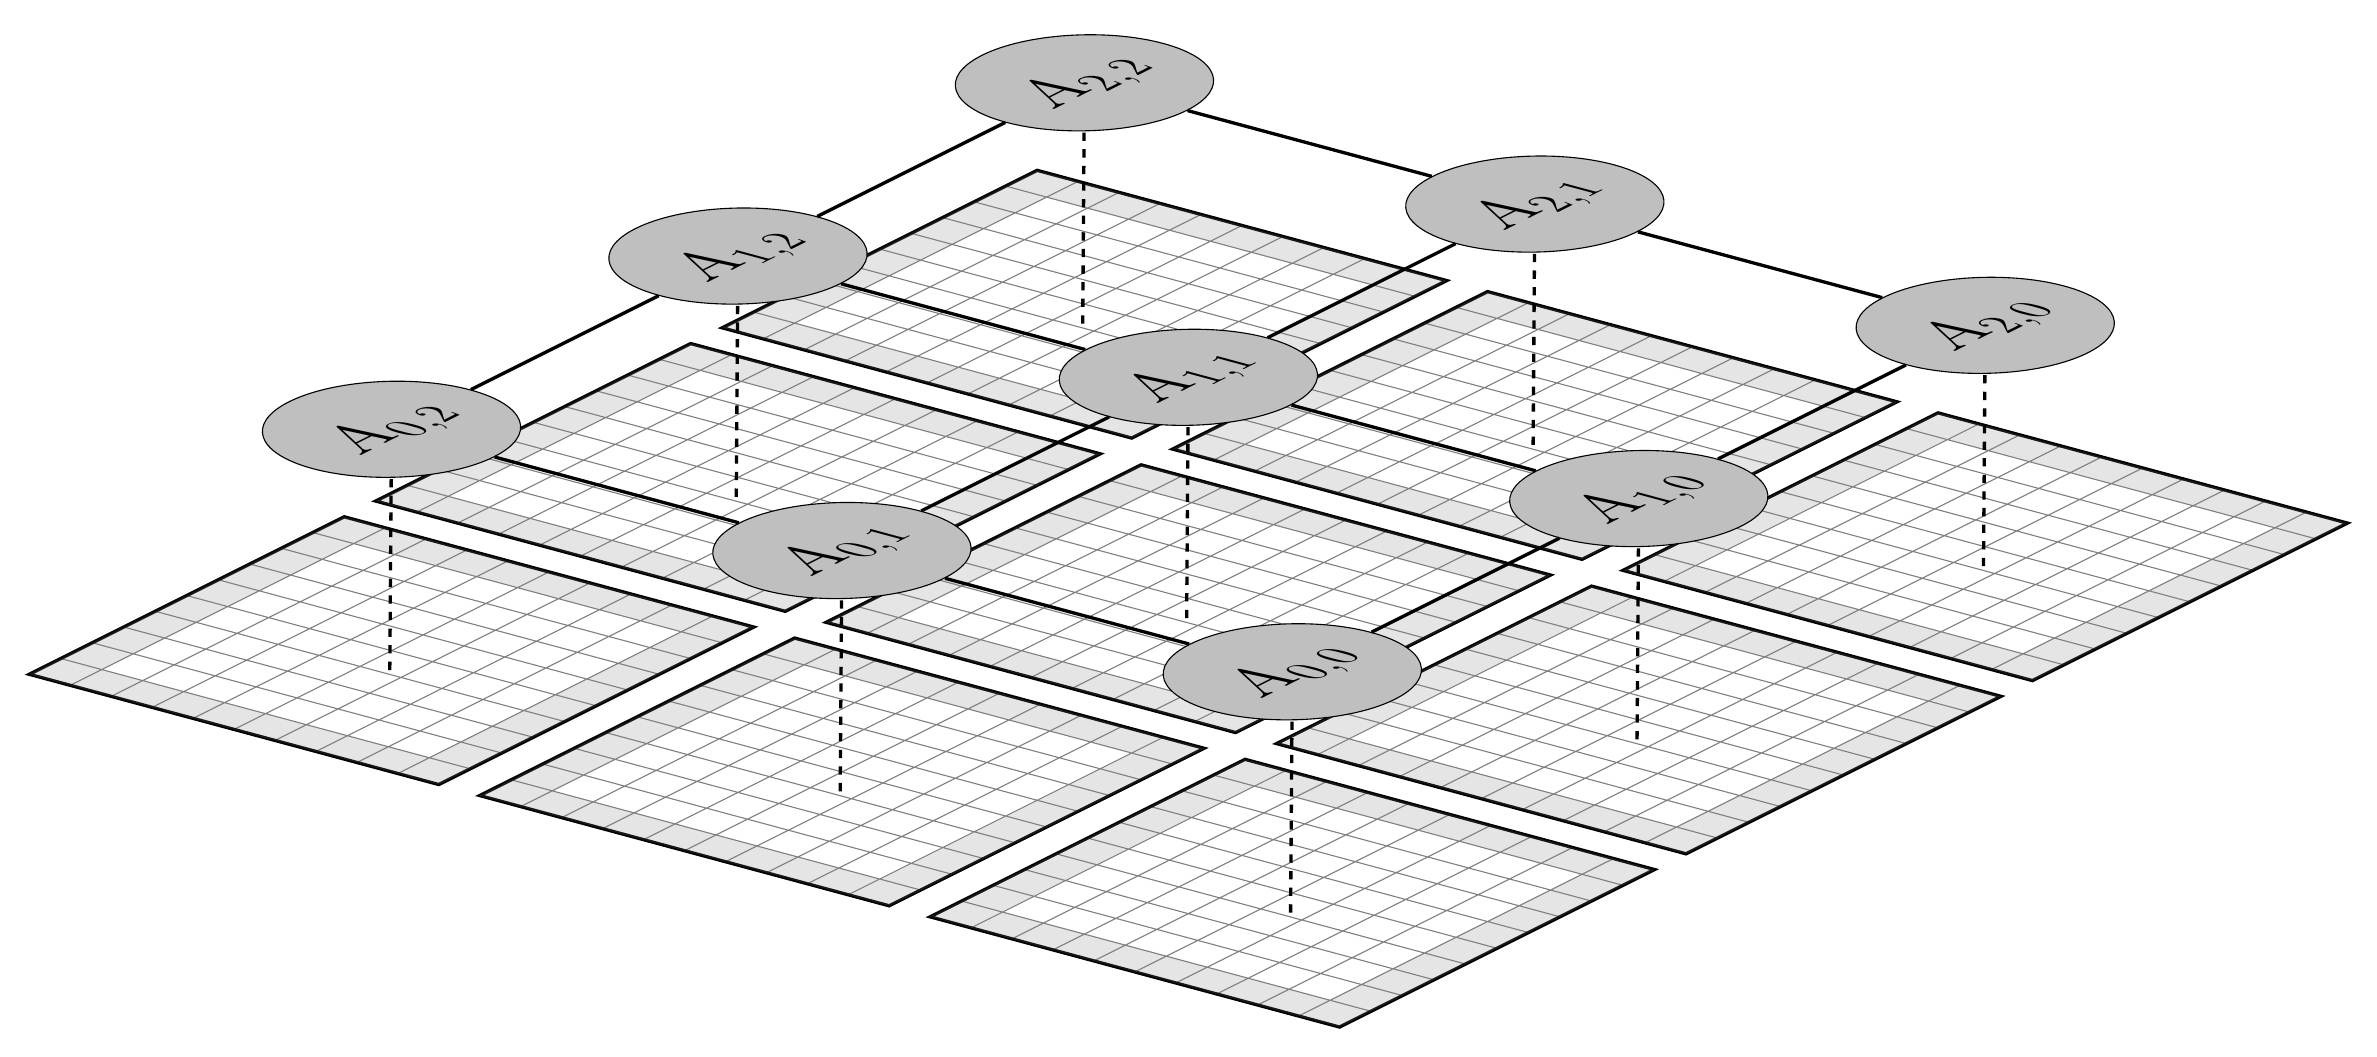
\begin{tikzpicture}[scale=2,
            every node/.style={minimum size=2cm},
            on grid
        ]
            % Grids
            \begin{scope}[
                    yshift=-100,every node/.append style={yslant=0.5,xslant=-1.3},
                    yslant=0.5,
                    xslant=-1.3
                ]
                \foreach \i in {0,1,2} {
                    \foreach \j in {0,1,2} {
                        \fill[white,fill opacity=0.9] (\i*2.2,\j*2.2) rectangle (2.2*\i+2,2.2*\j+2);
                        \draw[step=2mm, thin, gray] (\i*2.2,\j*2.2) grid (2.2*\i+2,2.2*\j+2);
                        \draw[black, very thick] (\i*2.2,\j*2.2) rectangle (2.2*\i+2,2.2*\j+2);
                        \fill[gray, opacity=0.2](\i*2.2,\j*2.2) rectangle (\i*2.2+2,\j*2.2+0.2);
                        \fill[gray, opacity=0.2](\i*2.2,\j*2.2+1.8) rectangle (\i*2.2+2,\j*2.2+2);
                        \fill[gray, opacity=0.2](\i*2.2,\j*2.2+0.2) rectangle (\i*2.2+0.2,\j*2.2+1.8);
                        \fill[gray, opacity=0.2](\i*2.2+1.8,\j*2.2+0.2) rectangle (\i*2.2+2,\j*2.2+1.8);
                    }
                }
            \end{scope}
            % Actors
            \begin{scope}[
                    yshift=-60,
                    %xshift=-20,
                    every node/.append style={yslant=0.5,xslant=-1.3},
                    yslant=0.5,
                    xslant=-1.3
                ]
                \foreach \i in {0,1,2} {
                    \foreach \j in {0,1,2} {
                        \draw [black, very thick, dashed] (2.2*\i+1,2.2*\j+1) -- (2.2*\i-1,2.2*\j-0.53);
                        \node [shape=circle, draw=black, fill=lightgray](A\i\j) at (2.2*\i+1, 2.2*\j+1){\huge$A_{\i,\j}$};
                    }
                }
                \foreach \i in {0,1,2} {
                    \foreach \j in {0,1,2} {
                        \pgfmathtruncatemacro{\top}{\j-1}
                        \pgfmathtruncatemacro{\left}{\i-1}
                        \ifthenelse{\j>0}{\path [very thick] (A\i\top) edge (A\i\j);}{}
                        \ifthenelse{\i>0}{\path [very thick] (A\left\j) edge (A\i\j);}{}
                    }
                }
            \end{scope}
        \end{tikzpicture}
    }
    \caption{Decomposition of the simulation domain into $3\times3$ blocks. Each block is assigned an actor that communicates the necessary data with its neighbors.}
    \label{fig:impl:actor_grid_mapping}
\end{figure}

In \autoref{fig:impl:actor_grid_mapping}, this behavior is illustrated via an actor graph with $3\times3$ actors.
The connection between two actors is signified by a single edge.
This connection is realized by four channels in the actual implementation, one pair of channels (incoming and outgoing) to exchange simulation data and another pair to exchange control messages, such as termination notices.
In \autoref{fig:impl:actor_graph}, the same actor graph is shown with all channels and their capacities visible.
The capacity of the channel needs to be at least two to avoid deadlocks due to non-consumed tokens. 
It does not have to be larger either due to the circular dependencies between the individual actors.

\begin{figure}
    \centering
    \resizebox{0.9\columnwidth}{!}{
        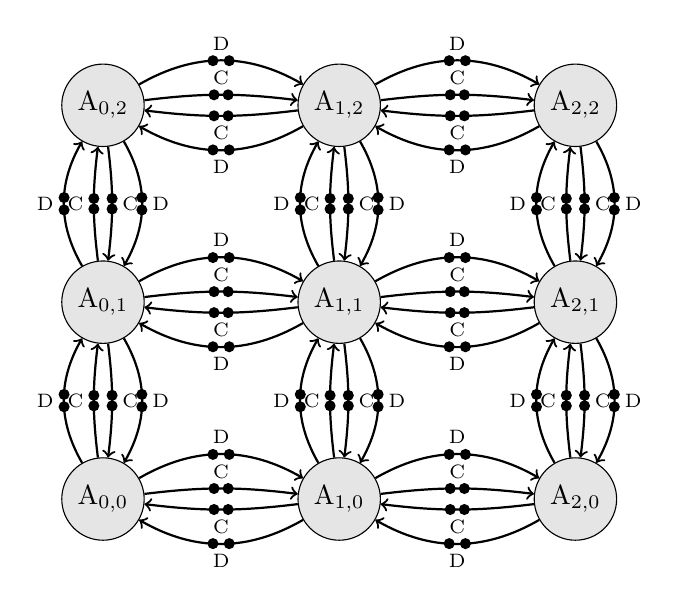
\begin{tikzpicture}
            \foreach \i in {0,1,2} {
                \foreach \j in {0,1,2} {
                    \node [shape=circle, draw=black, fill=lightgray!40] (A\i\j) at (3*\i,2.5*\j) {$\operatorname{A}_{\i,\j}$};
                }
            }
            \foreach \i in {0,1,2} {
                \foreach \j in {0,1,2} {
                    \pgfmathtruncatemacro{\top}{\i-1}
                    \pgfmathtruncatemacro{\bottom}{\i+1}
                    \pgfmathtruncatemacro{\left}{\j-1}
                    \pgfmathtruncatemacro{\right}{\j+1}
                    
                    % Data Channels
                    \ifthenelse{\j>0} {\path [->, thick] (A\i\j) edge [bend left] node[pos=0.45] {\tikz \fill circle(2pt);} node[pos = 0.55]  {\tikz \fill circle(2pt);} node[right] {\scriptsize D} (A\i\left);}{}
                    \ifthenelse{\i>0} {\path [->, thick] (A\i\j) edge [bend left] node[pos=0.45] {\tikz \fill circle(2pt);} node[pos = 0.55]  {\tikz \fill circle(2pt);} node[below] {\scriptsize D} (A\top\j);}{}
                    \ifthenelse{\i<2} {\path [->, thick] (A\i\j) edge [bend left] node[pos=0.45] {\tikz \fill circle(2pt);} node[pos = 0.55]  {\tikz \fill circle(2pt);} node[above] {\scriptsize D} (A\bottom\j);}{}
                    \ifthenelse{\j<2} {\path [->, thick] (A\i\j) edge [bend left] node[pos=0.45] {\tikz \fill circle(2pt);} node[pos = 0.55]  {\tikz \fill circle(2pt);} node[left] {\scriptsize D} (A\i\right);}{}
                    
                    % Control Channels
                    \ifthenelse{\j>0} {\path [->, thick] (A\i\j) edge [bend left=7] node[pos=0.45] {\tikz \fill circle(2pt);} node[pos = 0.55]  {\tikz \fill circle(2pt);} node[right] {\scriptsize C} (A\i\left);}{}
                    \ifthenelse{\i>0} {\path [->, thick] (A\i\j) edge [bend left=7] node[pos=0.45] {\tikz \fill circle(2pt);} node[pos = 0.55]  {\tikz \fill circle(2pt);} node[below] {\scriptsize C} (A\top\j);}{}
                    \ifthenelse{\i<2} {\path [->, thick] (A\i\j) edge [bend left=7] node[pos=0.45] {\tikz \fill circle(2pt);} node[pos = 0.55]  {\tikz \fill circle(2pt);} node[above] {\scriptsize C} (A\bottom\j);}{}
                    \ifthenelse{\j<2} {\path [->, thick] (A\i\j) edge [bend left=7] node[pos=0.45] {\tikz \fill circle(2pt);} node[pos = 0.55]  {\tikz \fill circle(2pt);} node[left] {\scriptsize C} (A\i\right);}{}
                }
            }
        \end{tikzpicture}
    }
    \caption{Actor graph for a simulation run with $3\times3$ actors. Each edge in the graph represents one channel. The number of black circles on a channel reflects its capacity. 
    The data type is denoted by C (control information) and D (copy layer data).}
    \label{fig:impl:actor_graph}
    %\vspace{-4mm}
\end{figure}

\subsection{Coordination via an actor-based run loop}
SWE-X10 follows the execution model imposed by the ActorX10 library.
For regular time steps, we follow the model introduced in \autoref{sec:actor:example}.
As shown above, the actor is connected using two channels, one for incoming and one for outgoing data.
Coordination is also similar: Every incoming border triggers the act method, but the update will only be triggered once all necessary updates are available and there is enough space in the channels to which the updates are written.
When no updates are needed, for example if none of an actor's neighbors is active, the method will trigger itself, until one of the neighbors becomes active.

\begin{figure}
    \centering
    \includegraphics[width=0.8\columnwidth]{figure/delayed_combined}
    \caption{Simulation run with $8\times8$ actors using lazy activation. 
    As the wave propagates (starting in the lower-left corner), more and more actors become active. 
    Dark blue patches represent ``lazy'' patches; lighter patches are active.}
    \label{fig:impl:example}
\end{figure}

As already explained, the simulated solution will remain in its initial steady state until the propagating wave initiated by an initial disturbance will arrive. 
We avoid superfluous computations on respective patches by assigning each actor an attribute that stores its activity status.
Initially, the status of each actor is set based on the scenario's initial condition. 
In many cases, the initial perturbation of the steady state will be restricted to a few patches, while the rest of the domain remains at rest.

\autoref{fig:fsm} gives an example for the FSM-based coordination.
As a first step, all actors in the simulation send their activity status to their neighbors using the control channels (sendActivation()).
Actors that contain part of this initial perturbation are set to the state \emph{propagating-wave}, while the rest is set to \emph{lake-at-rest}.
Then, active actors perform the simulation steps (computeStep()) once they receive all necessary updates ($recvActive()$).
During computation of the update, the patch determines for each of its copy layers whether the update actually changes any values.
If changes occurred or if the neighboring actor is already active, the updated layer will be sent.
If the neighbor is still inactive, the actor will also send a control message stating that updates are now available (sendActivation()).
Upon receiving the message ($recvActivation()$), the neighbor in the \emph{lake-at-rest} state will set itself to \emph{propagating-wave} and send its new activity status to all neighbors (sendStatus()), so that other neighbors that are already active can also start sending updates to the newly active actor.
Finally, once an actor has reached the termination condition, it will send a termination signal (sendTerm()) to other actors, which will be propagated until no more actors are active ($recvTerm()$).

\begin{figure}
    \resizebox{\columnwidth}{!}{
        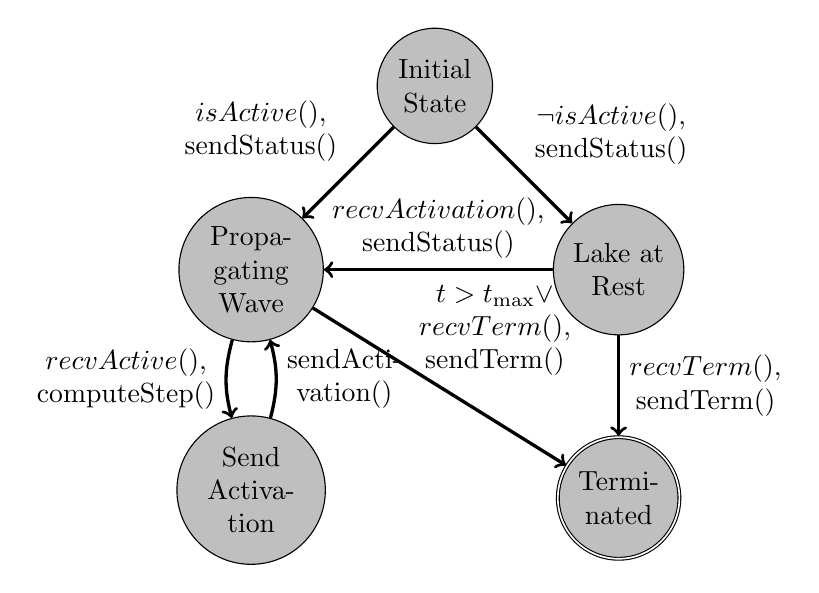
\begin{tikzpicture}
            \node [state, draw=black, fill=lightgray, align=center, node distance = 2.3cm] (initial) {Initial\\State};
            \node [state, draw=black, fill=lightgray, align=center, below right of = initial, node distance = 3.3cm] (rest) {Lake at\\Rest};
            \node [state, draw=black, fill=lightgray, align=center, below left of = initial, node distance = 3.3cm] (propagating) {Propa-\\gating\\Wave};
            \node [state, draw=black, fill=lightgray, align=center, below of = propagating, node distance = 2.8cm] (send) {Send\\Activa-\\tion};
            \node [accepting, shape=circle, draw=black, align=center, fill=lightgray, below of = rest, node distance = 2.9cm] (terminated) {Termi-\\nated};

            \path [->, very thick] (initial) edge node [above right, align=center]{$\neg isActive()$,\\sendStatus()} (rest);
            \path [->, very thick] (initial) edge node [above left, align=center] {$isActive()$,\\sendStatus()} (propagating);
            \path [->, very thick, bend right=15] (propagating) edge node [left, align=center] {$recvActive()$,\\computeStep()} (send);
            \path [->, very thick] (propagating) edge node [above right, align=center, xshift=-4mm] {$t>t_{\text{max}}\vee$\\$recvTerm()$,\\sendTerm()} (terminated);
            \path [->, very thick, bend right=15] (send) edge node [right, align=center] {sendActi-\\vation()} (propagating);
            \path [->, very thick] (rest) edge node [right, align=center] {$recvTerm()$,\\sendTerm()} (terminated);
            \path [->, very thick] (rest) edge node [above, align=center] {$recvActivation()$,\\sendStatus()}  (propagating);
        \end{tikzpicture}
    }
    \caption{Finite State machine for the simulation actor. Methods written in italics are guard functions, and functions written in normal letters are actions.}
    \label{fig:fsm}
\end{figure}

%\paragraph{Outlook on Adaptivity and Local Time Stepping}

In future work, we plan to implement block adaptivity and, as related functionality, a (multi-rate) local time-stepping scheme.
Both will make use of the FSM semantics provided by the actor model.
For example, when an actor is communicating with another actor running with only half of the time step size (due to higher resolution, e.g.), then it may use two separate states to deal with ghost layer data: 
one state for steps where a communication is needed and another state when the previously received data needs to be interpolated.
%
Block adaptivity will especially make load balancing more complicated.
Actors with a highly refined grid will have a significantly higher computational load. 
Hence, we will either need to allow splitting of actors, and allow actors to have more than one neighbor in each direction. 
Or we could make the assignment of actors to patches and cores more flexible and, for example, assign several cores (maybe even on accelerators) to the computation of refined patches. 

\subsection{Performance considerations}

The translation of X10 to machine code is a two-step process.
First, X10 code is compiled down to GNU C++. 
Then, the generated C++ code is translated down to machine instructions.
This two-step process and the research character of X10 lead to a number of interesting performance pitfalls.
Some of them, such as a lack of an available expression analysis, can be traced back to the two-step compilation process~\cite{horie2015rose}.
In the X10 compiler, the implementers focus on high-level optimizations specific to language features of X10, and leave the more standard optimizations to be done by the C++ compiler on the generated code.
However, the generated C++ code may be too complicated for the compiler to recognize optimizable patterns.
For example, the X10 array access \lstinline{val b = a(3)} translates to:
\begin{lstlisting}
x10_double b = (__extension__ ({
    ;
    x10_double ret6171;
    ret6171 = (a->FMGL(raw))->__apply(((x10_int)3));
    ret6171;
}))
\end{lstlisting}
%
All of these function calls are inlined by the C++ compiler at a later stage of the compilation, however, optimization steps executed prior to inlining will disregard the array access due to the complicated structure of the access\footnote{The optimization of function calls is complicated in C++, as the code of the function may not be available to the compiler, and it is difficult to rule out side effects.}~\cite{horie2015rose, grove2011performance}.
This is especially problematic in an HPC context.
%A common technique to obtain a speedup is to use SIMD instructions on potentially data-parallel sections of code. 
Auto-vectorization, for example, relies on the compiler to find code sections where loops may be transformed to exploit SIMD instructions.
Compilers rely on certain dependency patterns to infer that a vectorization of the code is possible.
In our tests, we found that the hot spots of our application, the solution of the edge-local Riemann problems on the unknown arrays was not vectorized by the compiler, though previous work 
showed successful auto-vectorization using C++~\cite{bader2014vectorization}.

Another, related problem are heap allocations in hot spots of the simulation. 
In C/C++, one can allocate arrays on the stack (e.g. \lstinline{float a[4];}) to store intermediate values in more extensive computations. 
In X10, the most primitive array type is the class \texttt{Rail}, a one-dimensional, zero-based, fixed-size storage for instances of a type.
As class instances, they are typically heap-allocated.
A naive port of the Riemann solver to X10 with Rail objects causes the overall runtime of the application to be dominated by the heap allocations made during the execution of the solver.
There is an annotation in X10 that guides the compiler to allocate the object on the stack instead, but we found that this did not improve the execution time by much.
We suspect secondary allocations to be responsible for that behavior.
One solution proposed before is to split small arrays of fixed size up into single variables to eliminate the stack allocations. 
While this technique reduced readability of the code, performance was greatly improved.

In SWE-X10, we decided to integrate native C++ code for the computational hot-spots of the simulation. 
Using the \texttt{@NativeRep} annotation, it is possible to skip the code generation process for an X10 class and to provide another implementation that matches the generated interface of the original X10 class instead.
That alternative implementation uses the dimensions provided by the \texttt{x10.regionarray.Array} object to iterate over the raw memory with a conventional loop nest and storing the unknowns of the simulation directly.
We assisted the compiler to generate vectorized code via \texttt{\#pragma simd} annotations.
Using state-of-the-art compilers (we used Intel C++ compiler 16.0 and Intel MPI), this is sufficient to obtain a more-than-4$\times$ speed-up over the non-vectorized, pure X10 version (see \autoref{sec:results}).

Another potential performance pitfall in the current implementation of X10 is the implicit capture of objects in \texttt{at (<PLACE>)}-statements.
Whenever a place-shift occurs, all objects referenced in the body of the statement are serialized and copied to the other place. 
A common mistake that leads to performance degradation in this context is the implicit capture of \texttt{this}.
This happens when a place-shift is performed in the body of an instance method and an instance member or another instance method of the object is accessed.
In both cases, the whole object (maybe an entire patch) including the complete object graph that is reachable from it will be copied, serialized and sent to the other place~\cite{grove2011performance}.

ActorX10 may be used to avoid some of these pitfalls.
Applications that comply with the ActorX10 execution model typically use the APGAS features of X10 for the application setup.
During the computation, however, different parts of the application only communicate via the channels defined initially, and no direct access to other actors' data is permitted.
Instead, all data transfers are performed through explicit library calls. 
A capture of \texttt{this} is not possible, as, in contrast to place-shifts, the member access expression is evaluated prior to the evaluation of the method call.
As long as the model is not violated, no implicit captures of \texttt{this} will happen during the execution of the actor-based computation~\cite{roloff2016actorx10}.

%\begin{itemize}
%    \item Split computation into patches, one actor per patch.
%    \item Four channels between every two neighboring actors.
%        \begin{itemize}
%            \item Incoming data
%            \item Outgoing data
%            \item Incoming Control messages
%            \item Outgoing control messages
%        \end{itemize}
%    \item Data exchange using Ghost layers.
%    \item Actor fires once updates from all neighbors are received.
%    \item lazy Activation of actors
%        \begin{itemize}
%            \item Actors exchange activity and boundaries initially. 
%            \item Actors save activity for each neighbor
%            \item Only send updates to active neighbors, only expect to receive from active neighbors.
%            \item when updates are first published to new boundary:
%                \begin{itemize}
%                    \item Sender: Send Activation message to activated neighbor
%                    \item Sender: Send Data to neighbor
%                    \item Newly activated: Set self to active, Mark Sender as active.
%                    \item Send activity to neighbors
%                    \item Newly activated: Send newly active message to all neighbors, active neighbors will now send to newly activated
%                    \item Newly activated: Normal time step: Send data to all active neighbors, ignore inactive patches for now.
%               \end{itemize}
%        \end{itemize}
%\end{itemize}

%%%%%%%%%%%%%%%%%%%%%%%%%%%%%%%%%%%%%%%%%%%%%%%%%%%%%%%%%%%%%%%%%%%%%%%%%%%%%%%%%%%%%%%%%%%%

\section{Results}
\label{sec:results}

We performed a battery of tests to evaluate the performance of SWE-X10.
Initially, we focused on the single-core performance with and without the native, vectorized solver.
Thereafter, we evaluated the differences in time-to-solution when actors are only activated gradually.
Finally, we evaluate the scaling behavior of our application in strong- and weak-scaling tests.

All tests were performed on the MAC Cluster (\url{http://www.mac.tum.de/wiki/index.php/MAC_Cluster}), a small cluster with (among others) 28 nodes equipped with two Intel Xeon E5-2670 CPUs (Sandy Bridge architecture) with a
peak performance of 332.8\,GFlop/s (single precision). The measured STREAM triad performance is 108.9\,GB/s per node. Nodes are connected through InfiniBand QDR.
We used the X10 Compiler in version 2.5.1 (MPI backend) and generated C++ code by Intel compiler 16.0.

\subsection{Benefits of vectorization}
\label{sec:results:vec}

The first test compares the floating point performance of pure X10 code against X10 code with native C++ code for the iteration over the unknowns of the domain, annotated with \texttt{\#pragma simd}.
In both cases, we use the HLLE solver. 
We performed tests on a single CPU core, with four actors and varying grid sizes.
The results are given in \autoref{fig:results:vec}.
As outlined in the following sections, the SWE-X10 implementation is on par with the C++-performance of the original SWE code.

\begin{figure}
    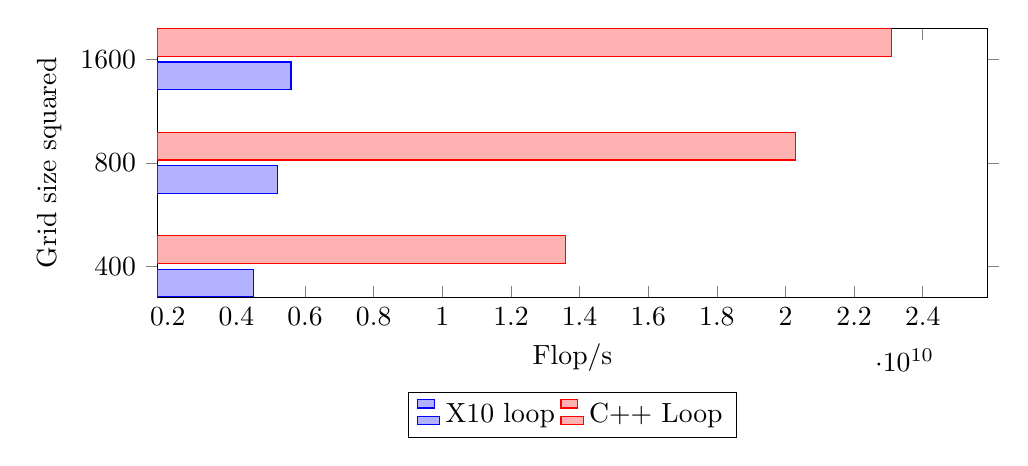
\begin{tikzpicture}
        \begin{axis} [
            symbolic y coords={400,800,1600},
            ytick=data,
            xlabel={Flop/s},
            ylabel={Grid size squared},
            enlargelimits=0.15,
            legend style={
                at={(0.5,-0.35)},
                anchor=north,
                legend columns=-1
            },
            xbar,
            width=\columnwidth, 
            height=5cm,
        ]
            \addplot coordinates {(4.49e9,400) (5.20e9,800) (5.59e9,1600)};
            \addplot coordinates {(1.36e10,400) (2.03e10,800) (2.31e10,1600)};
            \legend{X10 loop, C++ Loop}
        \end{axis}
    \end{tikzpicture}
    \caption{Performance of patch updates using an implementation in pure-X10 (blue) 
      vs.\ X10 with native, \texttt{pragma simd}-annotated C++-loops (red).}
    \label{fig:results:vec}
\end{figure}

\subsection{Single-node performance}
\label{sec:results:single-node}

In this section, we summarize the scaling behavior of SWE-X10 in terms of shared-memory parallelization,
as it was previously reported in an extended abstract~\cite{poeppl2016swex10}.
We performed a weak scaling test on a single node, and compared the results to SWE~\cite{breuer2012teaching,bader2014vectorization}, which is our corresponding reference implementation (using MPI+OpenMP and C++).
The setup for the benchmark is a radial dam break. Each CPU core holds a region of $1024\times1024$ cells, which is distributed onto $4$ actors with patches of size $512\times512$. 
We chose this configuration as it led to highest performance.
%As a comparison, we also performed the same computation with SWE~\cite{breuer2012teaching}, another solver for the shallow water equations based on OpenMP and MPI.

The performance for SWE-X10 and SWE for this test are shown in \autoref{fig:results:single-node}.
For SWE-X10, a single core reaches a performance of about 25\,GFlop/s. The performance plateaus at about 75\,GFlop/s from 10 cores, indicating a saturation of the memory bandwidth.
SWE ends up performing at the same level, however, it only saturates at a configuration with 14 cores.
In both cases, the codes manage to reach $23\,\%$ of the node's peak performance.

\begin{figure}
    \begin{tikzpicture}
        \begin{axis} [
                xlabel={CPU Cores},
                ylabel={GFlop/s},
                width=\linewidth,
                height=4cm,
                ymajorgrids=true,
                legend style={font=\scriptsize},
                legend pos=south east
        ]
        %\addplot [gray, domain=1:256] {x};
        \addplot+ [black, mark options={fill=black}] table [x=cores, y expr=\thisrow{flops}/1e9] {results/single-node.txt};
        \addplot+ [gray, mark options={fill=gray}] table [x=cores, y expr=\thisrow{comp-comm-flops}/1e9] {results/original-swe-single-node.txt};
        \legend{SWE-X10, SWE}
        \end{axis}
    \end{tikzpicture}
    \caption{Single-node performance of SWE-X10 (black) vs.\ SWE (gray). 
      We assigned four actors with $512\times512$ cells to each core (weak scaling). 
      The performance of SWE-X10 saturates earlier (10 cores) compared to SWE (14 cores),
     but both codes reach the same peak performance (75 GFlop/s). (Result from \cite{poeppl2016swex10})}
    \label{fig:results:single-node}
\end{figure}

\subsection{Multi-node performance}
\label{sec:results:multi-node}
To evaluate the multi-node performance of SWE-X10, we performed another weak-scaling test (shown previously in the extended abstract~\cite{poeppl2016swex10}).
In this test, each CPU (with eight cores) acted as one X10 place. 
Again 4 actors with $512\times512$ cells were assigned to each core, resulting in a total of 32 actors per CPU.
We executed the test for configurations ranging from one CPU up to sixteen nodes.
The achieved performance is shown in \autoref{fig:results:multi-node}.

From one to eight nodes ($2^4$ to $2^7$ cores), the performance scales linearly, but at sixteen nodes, a sublinear result was observed.
As the same performance degradation occurs with SWE, this may indicate a hardware issue.
%We are not sure about the cause of the problem, but suspect it may be due to performance fluctuations caused by thermal throttling on the MAC cluster.

In general, SWE-X10 performs better than SWE, which can be explained by the differing communication patterns used in the two software packages.
In SWE-X10, we implemented the actor-oriented approach, which is inherently concurrent and enables overlapping of computation with communication. An actor may update its patch while another actor communicates and is waiting for data, e.g.
In contrast, SWE uses a simple SPMD pattern, where computation and communication happen in phases, without overlap. 

\begin{figure}
    \begin{tikzpicture}
        \begin{loglogaxis} [
                xlabel={CPU Cores},
                ylabel={Flop/s},
                log basis x={2},
                width=\linewidth,
                height=4cm,
                legend style={font=\scriptsize},
                ymajorgrids=true,
                legend pos=north west
            ]
            \addplot+ [black, mark options={fill=black}] table [x=cores, y=flops] {results/weak-scaling-results.txt};
            \addplot+ [gray, mark options={fill=gray}] table [x expr= \thisrow{sockets} * 8, y=comp_comm_flops] {results/original-swe-weak.txt};
            \addplot [green, domain=8:256] {(9.27e10)/16*x};
            \legend{SWE-X10, SWE, Linear}
        \end{loglogaxis}
    \end{tikzpicture}
    \caption{Weak scaling of SWE-X10 (black) vs.\ SWE (gray) from one CPU ($2^3$ cores) 
      up to sixteen nodes ($2^8$ cores).
      32 actors with $512\times512$ cells were placed on each CPU. 
      The green line illustrates perfect scaling from one node. (Result from \cite{poeppl2016swex10})}
    \label{fig:results:multi-node}
\end{figure}

We conclude that the actor implementation in SWE-X10 allows favorable speed-up in shared and distributed memory, competitive to MPI+OpenMP implementations.

\subsection{Lazy activation of actors}
\label{sec:results:lazy}

In the following, we evaluate the benefit of lazy activation of patches using our actor approach. 
We cannot illustrate this benefit via reduced time-to-solution, yet, as this would require either load balancing among actors or migration of actors (incl.\ their patches) during run-time.
At the moment, actors are created and distributed to CPU cores at program-start. 
Migrating them to different cores or nodes is not possible yet. 
An alternative would be to migrate patches and assign them to actors on different cores or nodes. 
While this would reflect standard practice in HPC, it would substantially complicate the actor model: 
in particular, communication structures (i.e., channels between actors) would need to change dynamically. 
Such functionality is not yet implemented in ActorX10, and it will be part of our future research to evaluate the feasibility of such an approach. 

Hence, instead of time-to-solution, we measured the benefit of lazy evaluation by determining the CPU time (``CPU hours''), i.e.\ by summing up the time spent computing updates on each CPU.
This metric assumes that CPUs of inactive actors can remain (or be set to) an idle state, and allows a comparison of the amount of work (roughly reflecting the required energy) that is performed during program execution. 
In a resource-aware environment, it may be possible to activate CPU cores only when calculations actually commence.

\begin{figure}
    \centering
    \includegraphics[width=0.75\columnwidth]{figure/delayed_activation_test_setup}
    \caption{Setup to test lazy activation of actors. The red circle marks the initial water displacement.
    Throughout the simulation, it will collapse and radiate outwards as a propagating wave. 
    Each little square denotes an actor; the initial assignment of actors to places (i.e., CPUs), is marked in yellow.}
    \label{fig:results:lazy:setup}
\end{figure}

As a test setup, we again chose a radial dam break scenario with the dam break in the lower left corner of the scenario. 
Boundary conditions are set to wall type, and the simulation time is set to 90 simulated seconds.
We chose a grid resolution of $8192\times8192$ cells, distributed onto actors with patches of $512\times512$ cells each.
The actors were distributed across eight CPUs on four nodes of the MAC cluster, according to the scheme displayed in \autoref{fig:results:lazy:setup}.

We compared the CPU time with and without lazy activation.
For the run without lazy activation of patches, we obtained an overall execution time of 1,433 seconds. 
As all actors compute solutions from the start, and therefore all CPUs are used throughout the whole simulation, this sums up to 12,264 CPU seconds, or 3.41 CPU hours.

In comparison, the version with lazy activation takes 1,203 seconds to complete.
To obtain the aggregate CPU time, we logged the initial activation of the first actor for each place, from which we obtained the activation times displayed in \autoref{fig:results:lazy:result}
Summing over all active times yields an overall CPU time of 6,741 CPU seconds, or 1.87 CPU hours. 
Hence, in terms of total CPU time spent, we obtained a significantly lower use of computing resources. 

\begin{figure}
    \centering
    \label{fig:results:lazy:result}
    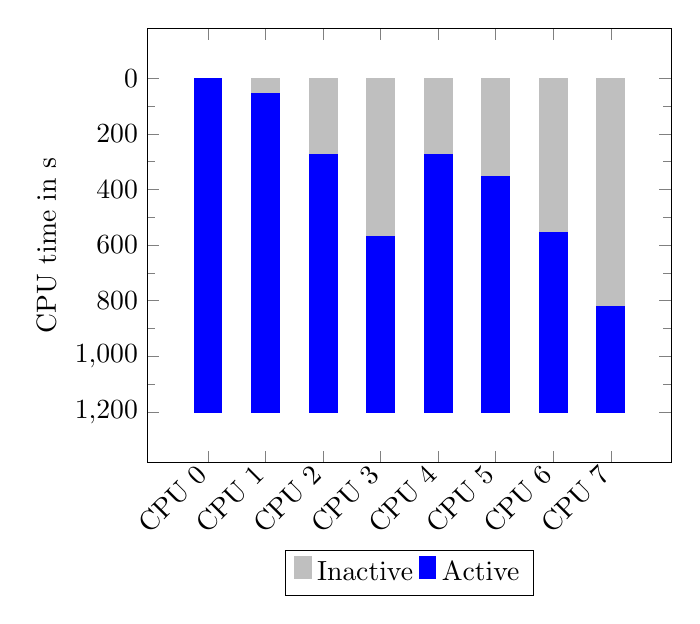
\begin{tikzpicture}
        \begin{axis} [ 
                ybar stacked, 
                enlargelimits=0.15, 
                legend style={
                    at={(0.5,-0.20)}, 
                    anchor=north,
                    legend columns=-1
                }, 
                ylabel={CPU time in s}, 
                symbolic x coords= {CPU 0,CPU 1,CPU 2,CPU 3,CPU 4,CPU 5,CPU 6,CPU 7}, 
                xtick=data, 
                x tick label style= {
                    rotate=45,
                    anchor=east
                }, 
                y dir=reverse,
                ytick={0, 200, 400, 600, 800, 1000, 1200},
                minor y tick num = 1,
                height = 7.1cm
            ] 
            \addplot+[ybar, lightgray] plot coordinates {(CPU 0, 0) (CPU 1, 52) (CPU 2, 272) (CPU 3, 566) (CPU 4, 272) (CPU 5, 351) (CPU 6, 551) (CPU 7, 819)};
            \addplot+[ybar, blue] plot coordinates {(CPU 0, 1203) (CPU 1, 1151) (CPU 2, 931) (CPU 3, 637) (CPU 4, 931) (CPU 5, 852) (CPU 6, 652) (CPU 7, 384)};

            \legend{Inactive, Active} 
        \end{axis} 
    \end{tikzpicture}
    \caption{CPU activity for the test run with lazy actor activation. Each bar represents the activity of one CPU; gray marks inactive time and blue marks time spent computing updates.}
\end{figure}

Note that the concrete gain of lazy activation of course depends heavily on the initial scenario.
In cases where the initial disturbance is in the center of the domain, gains will be significantly smaller.
Nevertheless, typical tsunami simulation setups for example, will feature comparably local initial disturbances and (esp.\ for simulation of far-field tsunamis at ocean-scale) large ``inactive'' domains during the first phase of a simulation.  
%However, there is no major drawback to the technique, and the computational overhead is minimal.

%\begin{itemize}
%    \item Comparison Vectorized vs. Unvectorized HLLE solver.
%    \item Single-node performance with and without lazy activation
%    \item Multi-node performance with and without lazy activation
%\end{itemize}

%\section{Related Work}
%\begin{itemize}
%    \item[\cite{breuer2012teaching}] Classic SWE. Basis for numerics, discretization and single-block implementation.
%    \item[\cite{bader2014vectorization}] Riemann solvers used in SWE-X10 are from there. Also provides performance results in comparable scenario.
%    \item[\cite{unterweger2015peanoclaw}] PeanoClaw. Adaptive mesh refinement instead of lazy activation. Space-tree approach
%    \item[\cite{roloff2016actorx10}] ActorX10 library.
%\end{itemize}
 
\section{Conclusion and Outlook}
\label{sec:conclusion}

%\todo{This is a rough sketch for the outlook. Much will probably be rewritten... Citations I will add too.}
In this paper, we presented first results of an actor-based solver for the shallow water equations, SWE-X10. 
We demonstrated high node-level performance (due to auto-vectorization of ``X10-native'' loops) and solid scalability that benefits from overlapping of computation and communication, exploiting the actor model. 
%a foundation and a very early state of the realization of our vision for the SWE-X10.
Currently, SWE-X10 only makes limited use of the flexibility provided by the actor model; 
we thus aim to expand SWE-X10 in two key directions: 
(1) an expansion towards block-adaptive mesh refinement together with local time stepping, 
%a dynamic splitting and joining of actors devoid of global coordination and local time stepping as one goal, 
and (2) the characterization of performance and respective improved scheduling in heterogeneous environments.

When using block-adaptive meshes with local time stepping, as in \cite{leveque2011tsunami}, multiple layers of meshes with different resolutions are used. 
Here, lazy activation may be enforced on the fine-level meshes, and dynamic deactivation needs to be offered by the actors' finite state machines. 
Any activation or deactivation of an actor then needs to trigger a load-balancing step:
based on a performance characterization of actor activities (as outlined in \autoref{sec:perfmodel}), 
actors may be migrated to other X10 places. 
Also, dynamic splitting of heavy-weight actors or merging of several light-weight actors should be considered to improve the granularity of parallelism, similar to \cite{weinzierl14block}.
Finally, an important goal is to implement (local) time stepping schemes (incl.\ actor-based load balancing) without a global coordination scheme, which are known to easily cause scalability bottlenecks. 

%In future work, we plan on implementing a local time-stepping scheme and, as related functionality, block-adaptivity.
%Both will make use of the finite state machine semantics the actor model provides us with.
%For example, when an actor is communicating with another actor that has a grid with only half of the time step size of this actor, then it may use one state for steps where a communication is needed and another for steps when the previously received data needs to be interpolated.
%Using the same scheme, it should also be possible to coordinate locally with neighboring actors of different resolutions.
%This adaptivity also complicates load balancing, however.
%In some cases, actors with a highly refined grid may have a computational load that is significantly higher than those of other actors, and in such cases, it may be advisable to split the actor into several actors sharing the work-load of the prior actor.
%On the other hand, it may be sensible to merge actors should their workload be too small compared to the other actors.

%The other aforementioned aspect deals with the complexity of finding suitable workload distributions for heterogeneous hardware configurations.
%After the end of Dennard-Scaling~\cite{???}, alternate ways to accelerate computations, such as GPUs, MIC accelerators, FPGAs, DSPs or programmable fabric have been proposed~\cite{???}.
%In many of the front-ranking clusters in the TOP500 list, GPUs or Xeon Phi accelerators are used alongside the classical CPUs.
%It will be an important for application developers in the field of high performance computing to use the capacities of these heterogeneous systems as thoroughly as possible.
%We aim to use design space exploration, a technique from the world of embedded computing~\cite{someglassthing} to characterize the optimal distribution of work amongst these parallel resources.

%%%%%%%%%%%%%%%%%%%%%%%%%%%%%%%%%%%%%%%%%%%%%%%%%%%%%%%%%%%%%%%%%%%%%%%%%%%%%%%%%%%%%%%%%%%%
%%%%%%%%%%%%%%%%%%%%%%%%%%%%%%%%%%%%%%%%%%%%%%%%%%%%%%%%%%%%%%%%%%%%%%%%%%%%%%%%%%%%%%%%%%%%
%% END MAIN MATTER
%%%%%%%%%%%%%%%%%%%%%%%%%%%%%%%%%%%%%%%%%%%%%%%%%%%%%%%%%%%%%%%%%%%%%%%%%%%%%%%%%%%%%%%%%%%%
%%%%%%%%%%%%%%%%%%%%%%%%%%%%%%%%%%%%%%%%%%%%%%%%%%%%%%%%%%%%%%%%%%%%%%%%%%%%%%%%%%%%%%%%%%%%
%
% The following two commands are all you need in the
% initial runs of your .tex file to
% produce the bibliography for the citations in your paper.
\bibliographystyle{abbrv}
\bibliography{literature}  % sigproc.bib is the name of the Bibliography in this case
% You must have a proper ".bib" file
%  and remember to run:
% latex bibtex latex latex
% to resolve all references
%
% ACM needs 'a single self-contained file'!
%
%APPENDICES are optional
%\balancecolumns
%\appendix
%Appendix A
\section*{ACKNOWLEDGEMENTS}
This work was supported by the German Research Foundation (DFG) as part of the Transregional Collaborative Research Centre ``Invasive Computing'' (SFB/TR 89).


%\balancecolumns % GM June 2007
\end{document}
